\documentclass[sigconf]{acmart}

% For ACM Conference format (already set by 'sigconf')
\usepackage{graphicx}
\usepackage{booktabs} % For professional tables

\begin{document}

\title{Analyzing GPU Multiprocess Service (MPS) Impact on Diverse Workloads}

\author{Anonymous}
\affiliation{\institution{Under Review}}

\begin{abstract}
NVIDIA's Multi-Process Service (MPS) enables concurrent kernel execution on GPUs, offering the potential for higher throughput. In this paper, we evaluate the impact of MPS across diverse CUDA workloads by designing targeted experiments that represent light, heavy, memory-bound, and saturated usage patterns. Through detailed measurement and analysis, we demonstrate the cases where MPS significantly improves performance, where it has marginal benefit, and where it even degrades performance. Our findings help practitioners decide when enabling MPS is advantageous.
\end{abstract}

\maketitle

\section{Introduction}

As deep learning, simulation, and high-performance applications increasingly rely on GPUs, sharing GPUs efficiently among multiple processes becomes critical. While CUDA streams allow some degree of overlap, NVIDIA's Multi-Process Service (MPS) offers a more powerful mechanism by enabling multiple processes to concurrently submit work to the GPU.

However, the effectiveness of MPS depends heavily on the nature of the workloads. In this paper, we systematically evaluate when MPS improves performance and when it may not be beneficial.

\section{Background: CUDA MPS}

MPS is designed to reduce kernel launch latency and allow fine-grained concurrent execution on GPUs. It virtualizes the device driver, allowing multiple user processes to behave like independent streams within a single process context.

Despite its promise, enabling MPS can introduce overheads, especially if workloads are lightweight, memory-bound, or saturate the GPU resources improperly.

\section{Methodology}

We implemented six CUDA workloads:
\begin{itemize}
    \item \textbf{vector\_add}: elementwise vector addition (light workload)
    \item \textbf{image\_convolution}: simple 2D convolution (light workload)
    \item \textbf{matrix\_mul}: dense matrix multiplication (heavy workload)
    \item \textbf{fft}: Fast Fourier Transform (heavy workload)
    \item \textbf{memory\_copy}: host-to-device and device-to-host transfers (memory-bound)
    \item \textbf{prefix\_sum}: inclusive scan operation (memory and compute mix)
\end{itemize}

We designed mixture experiments combining these workloads into different categories:
\begin{itemize}
    \item Light-Light (\texttt{vector\_add + image\_convolution})
    \item Heavy-Heavy (\texttt{matrix\_mul + fft})
    \item Memory-Compute (\texttt{memory\_copy + matrix\_mul})
    \item Memory-Memory (\texttt{memory\_copy + prefix\_sum})
    \item Saturated-Light (24 \texttt{vector\_add})
    \item Saturated-Heavy (24 \texttt{matrix\_mul})
\end{itemize}

All experiments were run with and without MPS, recording wall-clock execution times.

\section{Results}

\subsection{Light Workloads}

\begin{figure}[h]
    \centering
    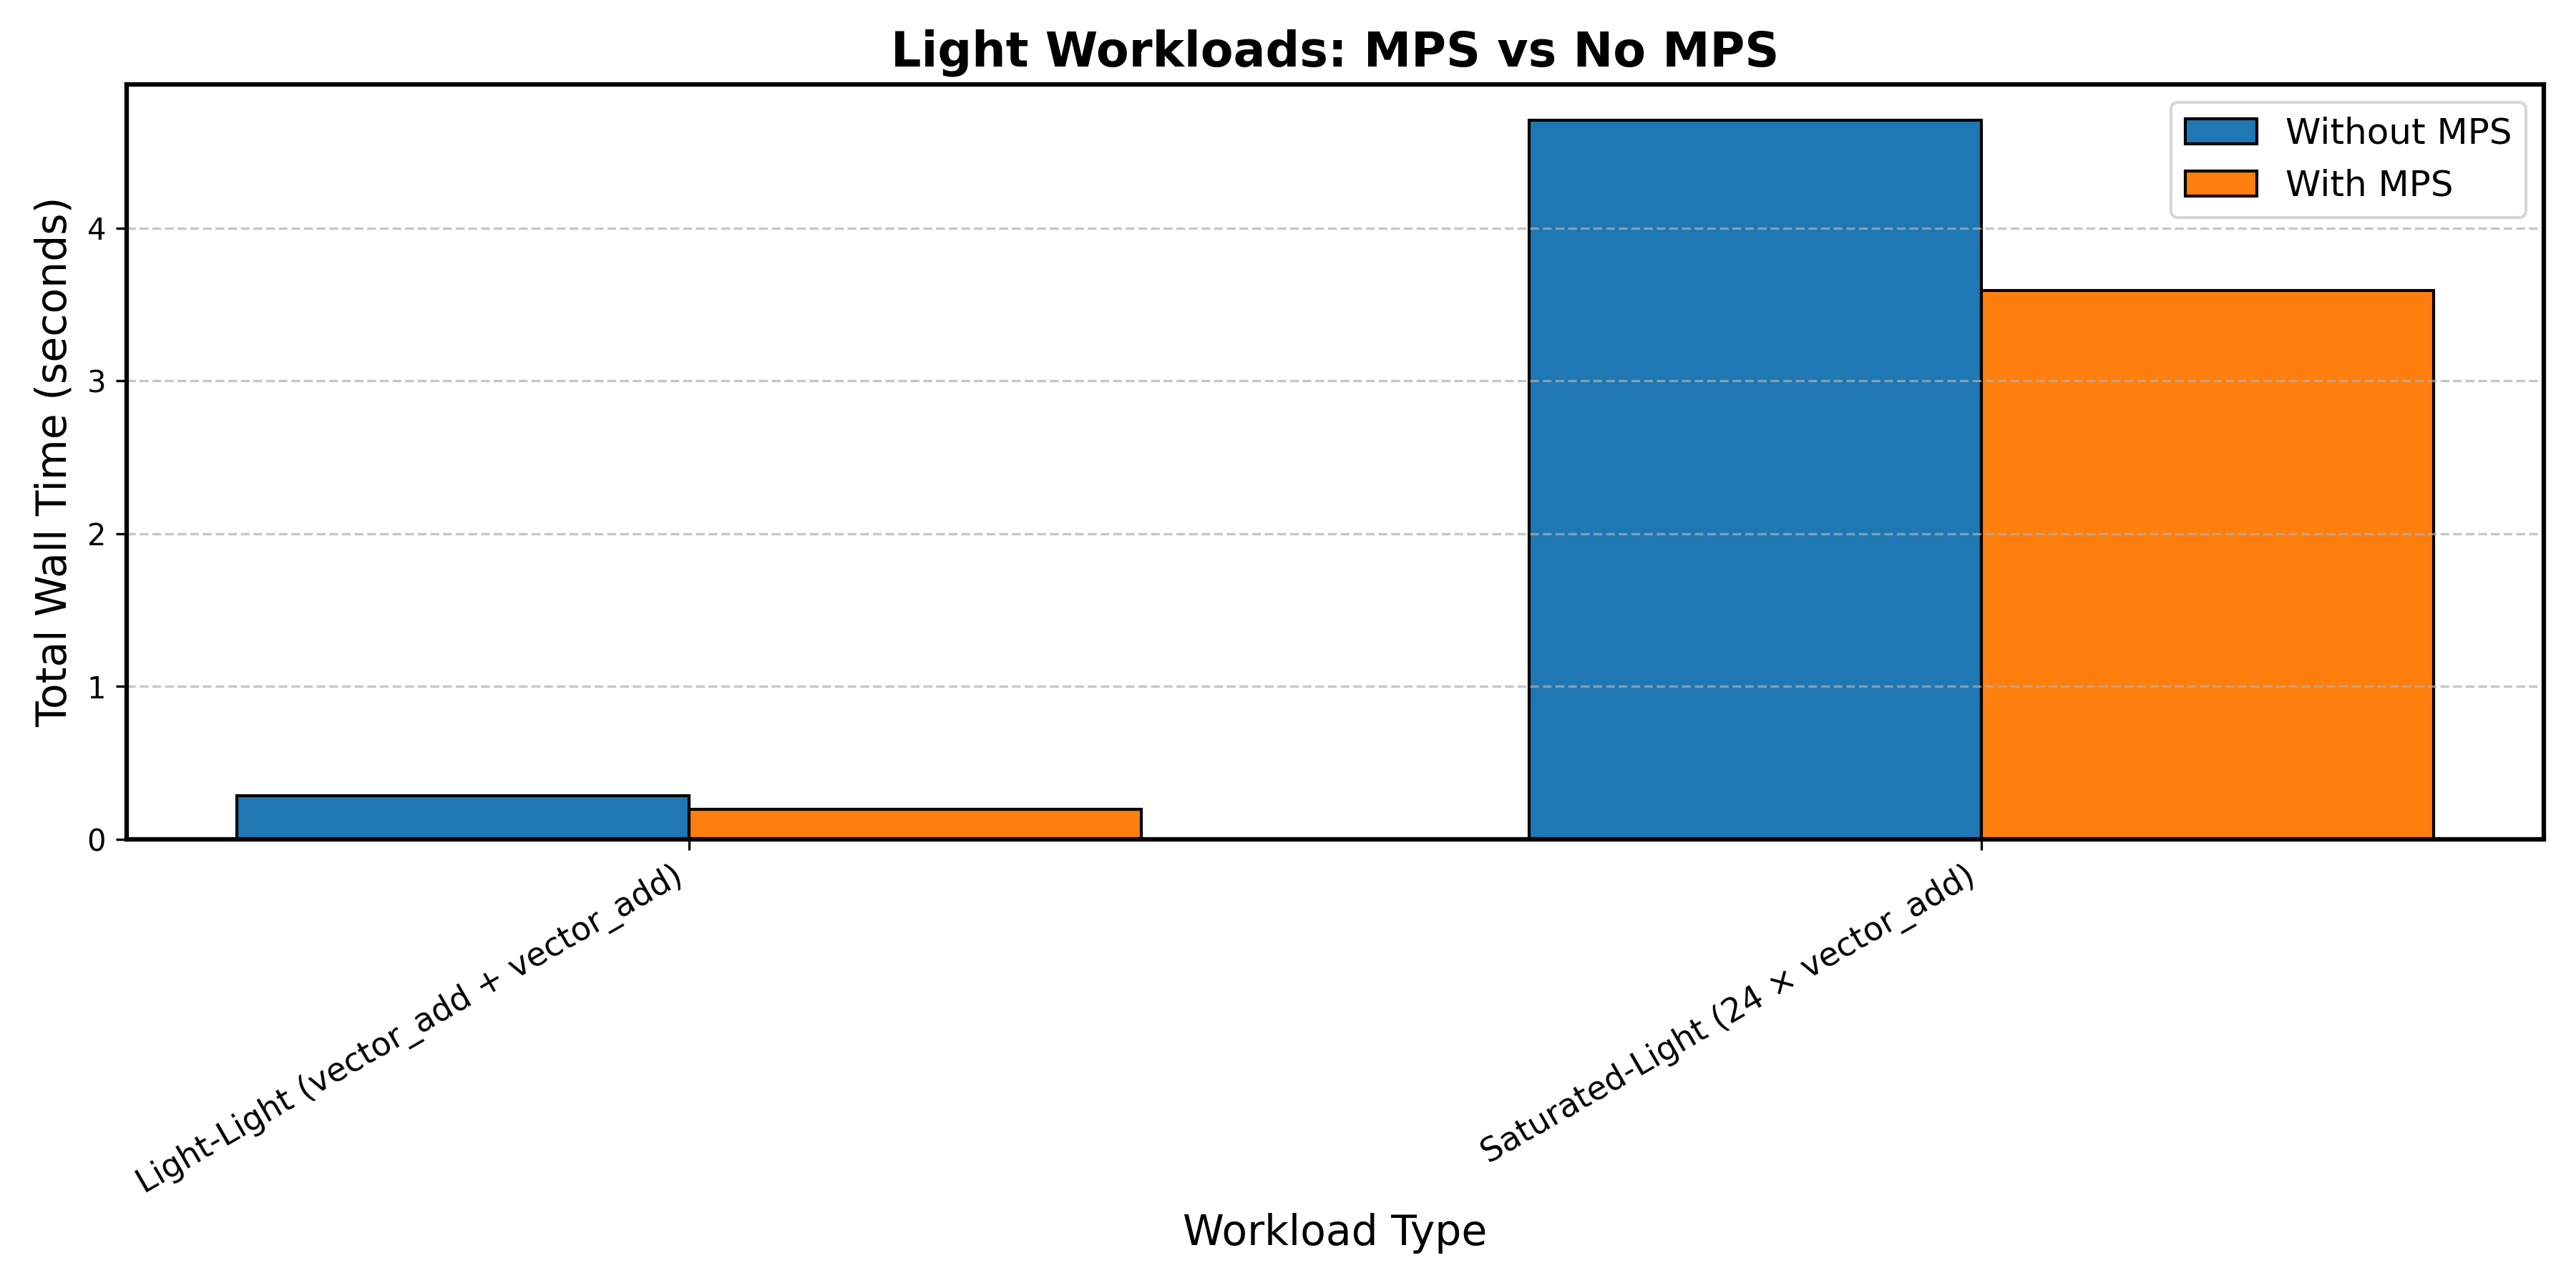
\includegraphics[width=\linewidth]{../plots/light_workloads.png}
    \caption{Light workloads (\texttt{vector\_add} + \texttt{image\_convolution}) and Saturated Light (24x \texttt{vector\_add}).}
    \label{fig:light_workloads}
\end{figure}

Figure~\ref{fig:light_workloads} shows that light workloads benefit moderately from MPS. Overhead can dominate when the kernels are extremely small.

\subsection{Heavy Workloads}

\begin{figure}[h]
    \centering
    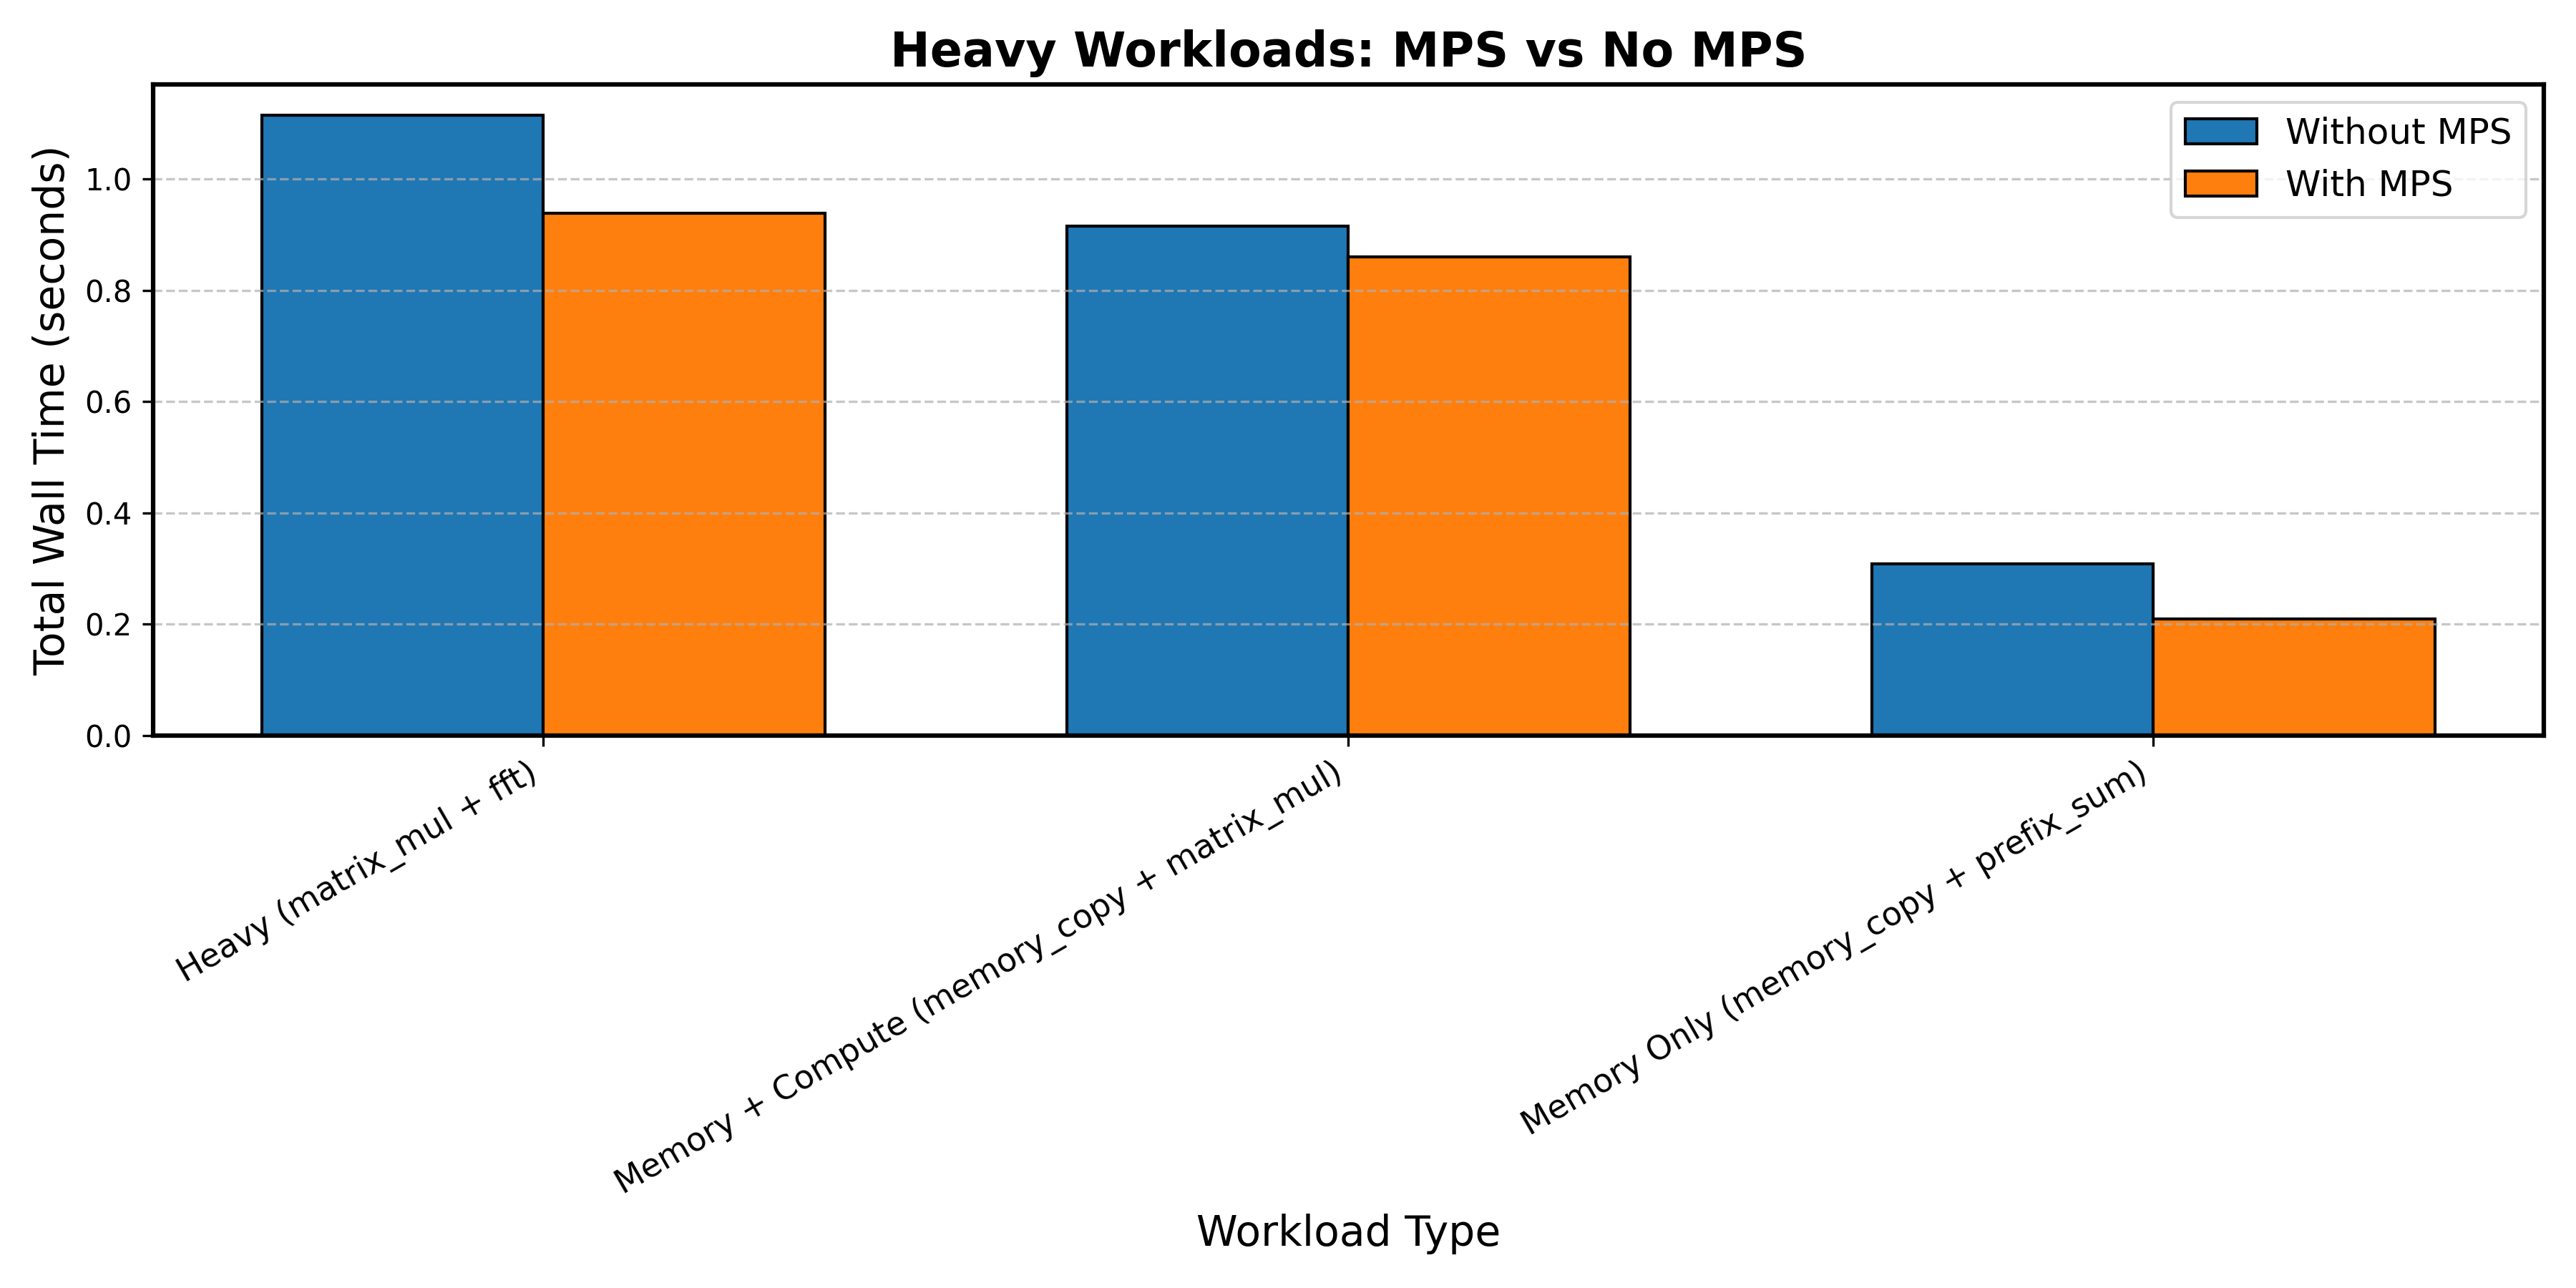
\includegraphics[width=\linewidth]{../plots/heavy_workloads.png}
    \caption{Heavy and memory-compute workloads.}
    \label{fig:heavy_workloads}
\end{figure}

As seen in Figure~\ref{fig:heavy_workloads}, heavy computational kernels such as matrix multiplication and FFT benefit significantly from MPS.

\subsection{All Mixtures Overview}

\begin{figure}[h]
    \centering
    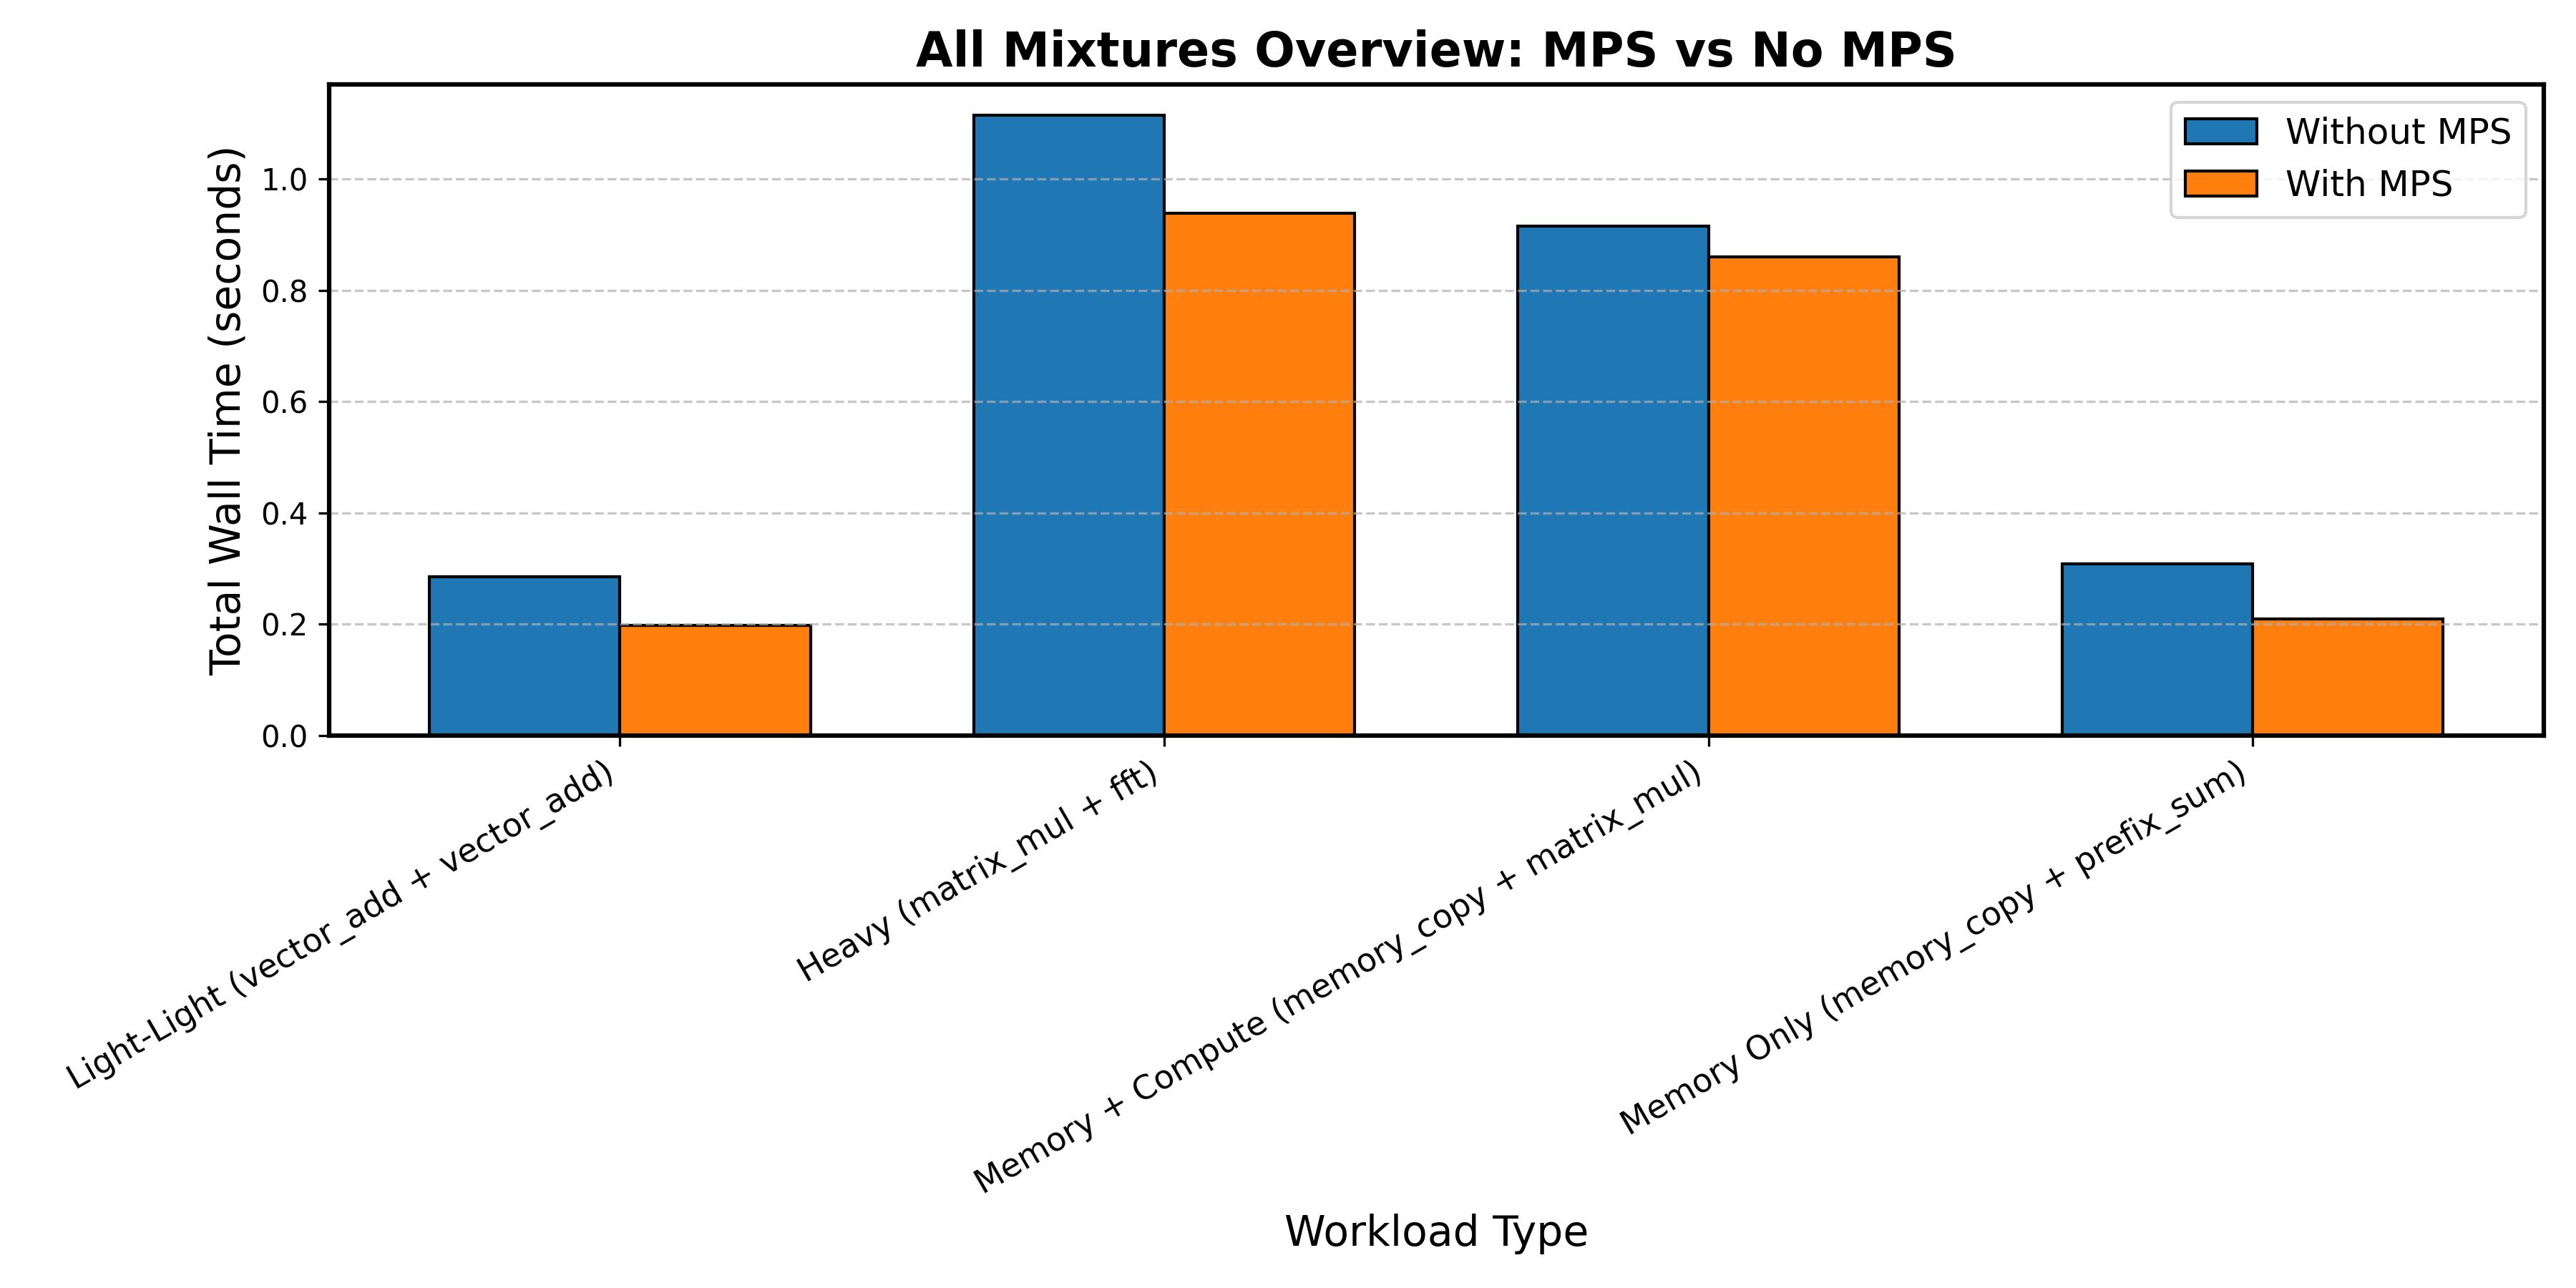
\includegraphics[width=\linewidth]{../plots/all_mixtures_overview.png}
    \caption{Overview of different mixture experiments.}
    \label{fig:all_mixtures}
\end{figure}

Figure~\ref{fig:all_mixtures} summarizes that MPS accelerates diverse workloads, with the greatest impact on compute-heavy and moderately memory-bound mixtures.

\subsection{Saturated Workloads}

\begin{figure}[h]
    \centering
    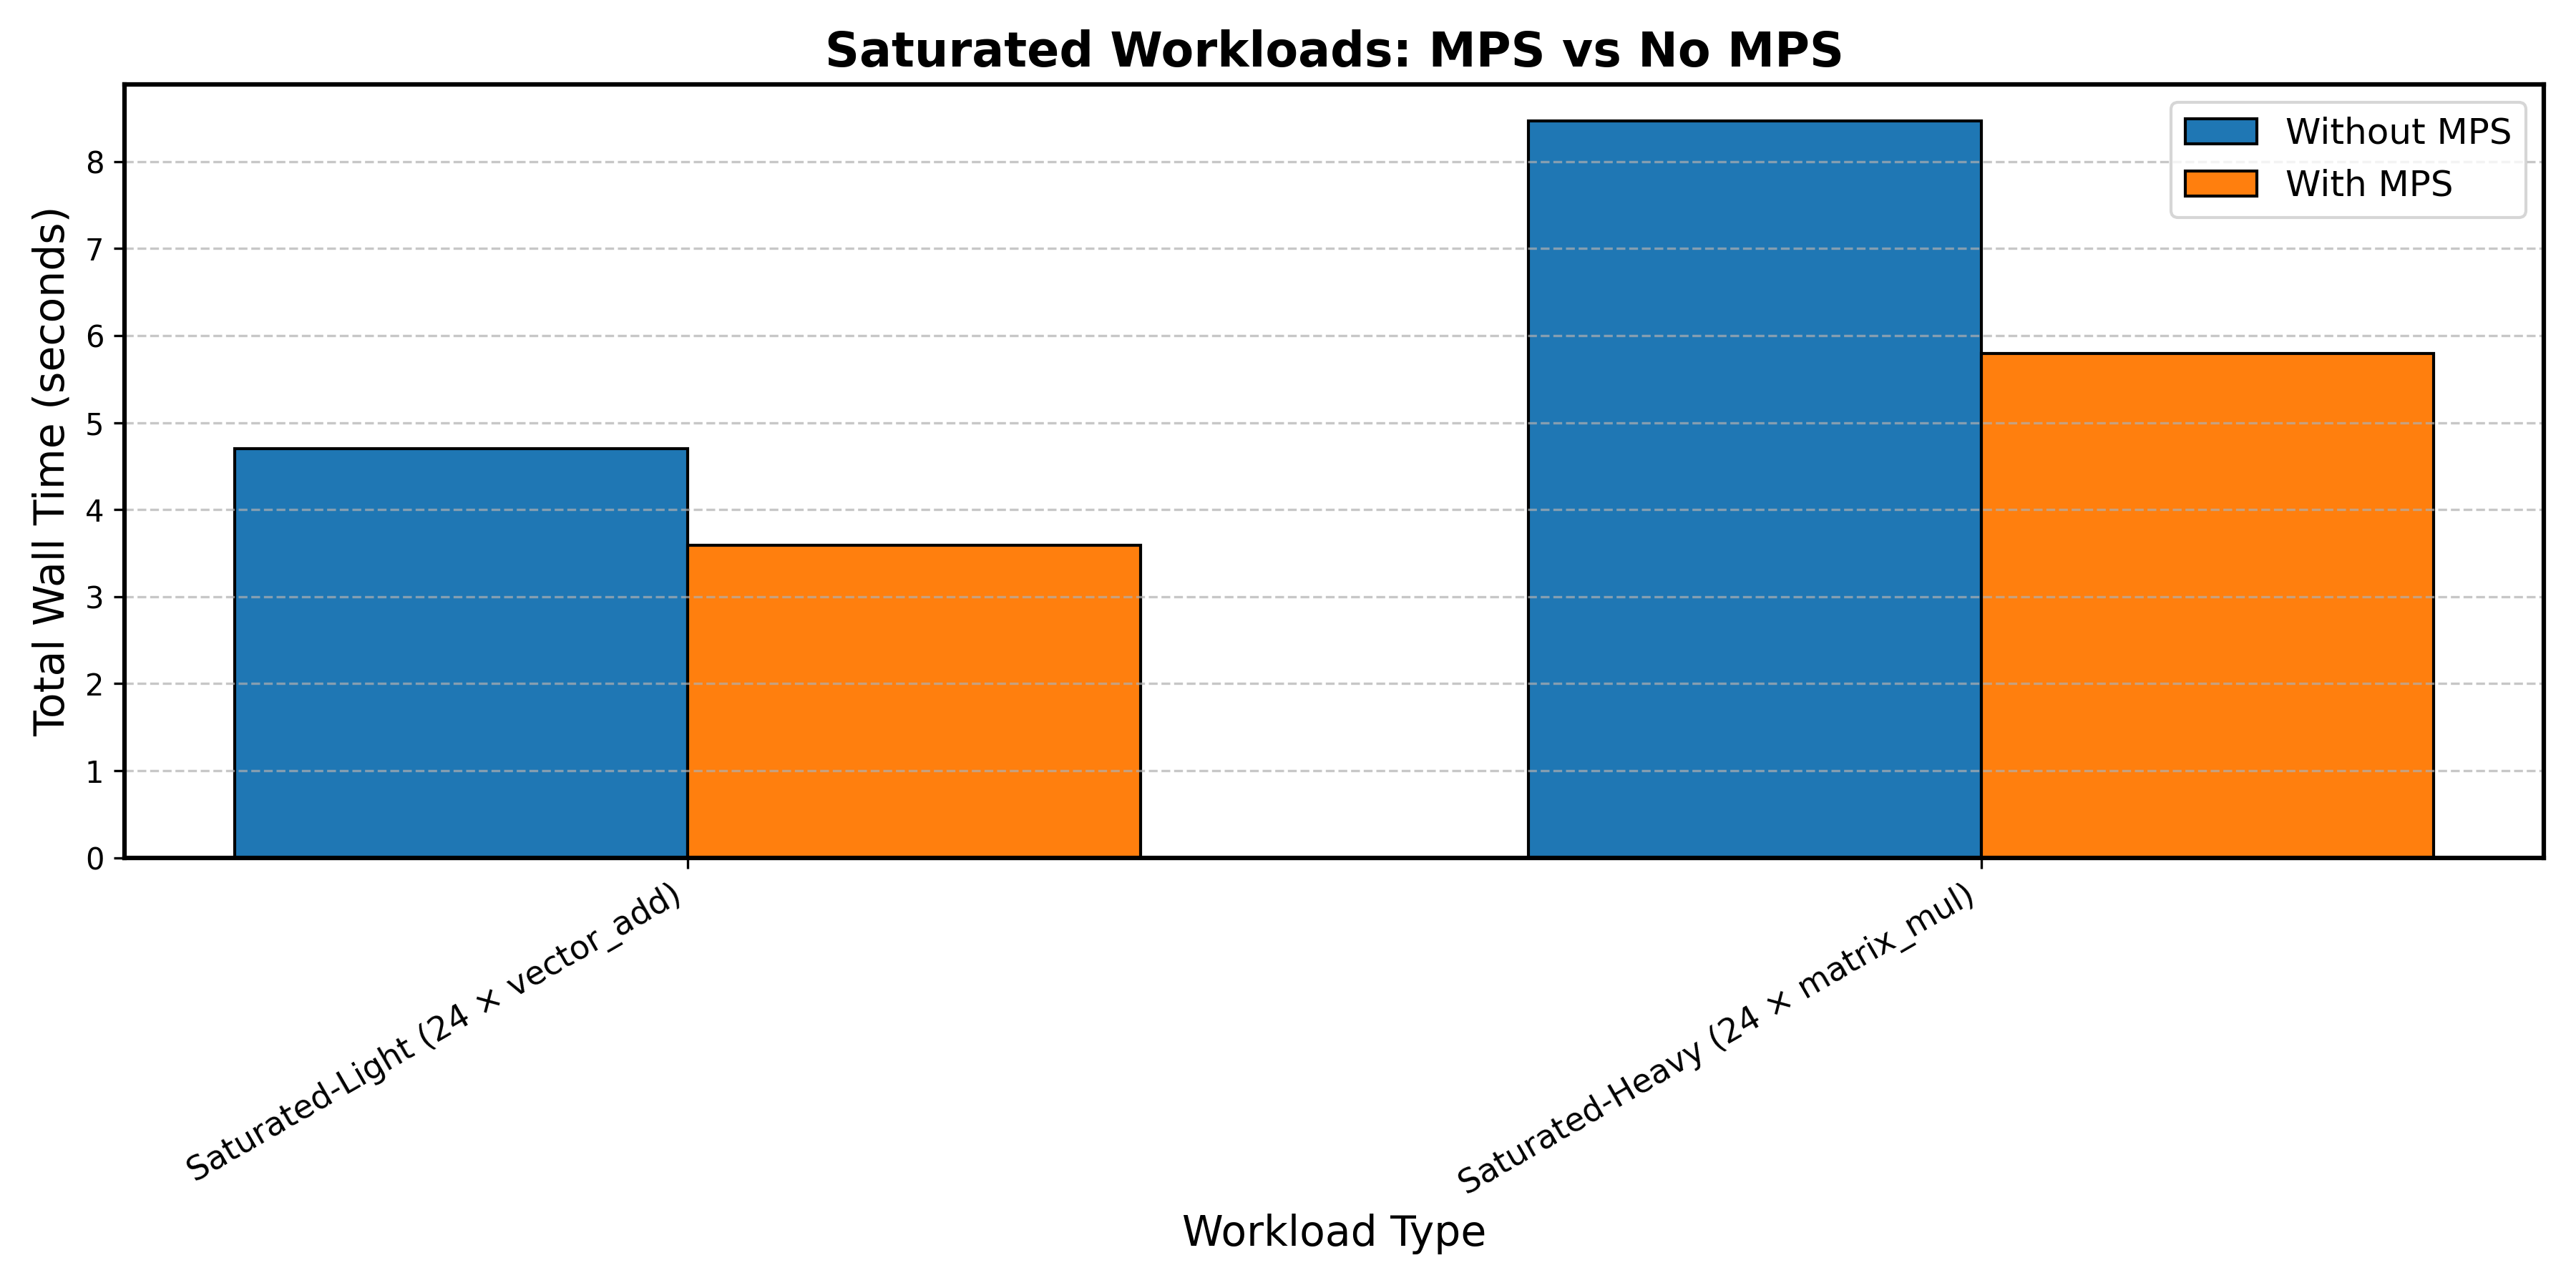
\includegraphics[width=\linewidth]{../plots/saturated_workloads.png}
    \caption{Highly saturated GPU workloads.}
    \label{fig:saturated}
\end{figure}

In Figure~\ref{fig:saturated}, saturated heavy workloads (24x matrix\_mul) show little gain, highlighting the limits of MPS when SM occupancy is already maximized.

\section{Discussion}

Our experiments reveal that:
\begin{itemize}
    \item \textbf{Light workloads}: benefit modestly, but overhead may offset gains.
    \item \textbf{Heavy workloads}: benefit significantly from concurrent kernel execution.
    \item \textbf{Memory-bound workloads}: show mixed results depending on balance.
    \item \textbf{Saturated workloads}: MPS helps little once resource limits are reached.
\end{itemize}

Thus, enabling MPS is most beneficial when multiple medium-to-heavy compute kernels are expected to execute together.

\section{Conclusion}

CUDA MPS is a powerful tool for boosting GPU throughput, but its impact is workload dependent. This study provides practical insights to guide developers in deciding when to leverage MPS for their serverless inference, HPC, or ML pipelines.

\bibliographystyle{ACM-Reference-Format}
\bibliography{../references}

\end{document}
